\chapter{Effects of Variation on the Evolution of Larval Trait Parameters}
The stochasticity in the model comes from the initial standing variation in the larval trait parameters as well as from the heritability of each trait parameter during the inheritance of those traits. The results from simulations show how these sources of variations play an important role in determining the evolutionary routes taken to inrease fitness and achieve greater competitive ability.
\section{Variation in the Initial Distribution of Larval Trait Parameters}
In the initial distribution of each trait value, the variation comes from the standard deviation given for each distribution of the traits like feeding rate, waste tolerance, critical size and efficiency. The initial standing variation in these trait distributions determine the maximum mean trait value that can be achieved to increase the fitness. Simulations were performed for given fixed mean trait values but varying their respective initial standing variation to see how these variations interact to obtain maximum fitness in multiple ways at $50^{th}$ generation. In fig~\ref{fig:ivar_fr_eff} - ~\ref{fig:ivar_mc_eff}, differences of the mean trait values of the population at $50^{th}$ generation and $0^{th}$ generation are plotted for different combinations of intial variation in trait values. The initial standard deviation for a trait is taken as a certain precentage of its respective mean trait value at $0^{th}$ generation. These initial conditions used in simulations are given in table (no.).\\\\
These results show that it is clear that differences in variation of these trait parameters give different mean trait values at $50^{th}$ generation across different crowding densities. Overall there is no significant effect of initial variation in trait parameters on the mean trait values in MB culture is found. Higher initial variation in initial feeding rate anf efficiency give higher mean initial feeding rate and mean efficiency respectively after $50^{th}$ generation in MCU and CCU cultures without interacting with each other (see fig~\ref{fig:ivar_fr_eff}). There is no difference in mean trait values
(initial feeding rate and efficiency) of MCU and CCU cultures. Initial feeding rate in MCU culture is lesser than in CCU culture only when initial variation is high and there is no interaction with variation in critical size at all densities (see fig~\ref{fig:ivar_fr_mc}). There is no significant effect on the mean critical size at $50^{th}$ generation due to initial variation initial feeding rate and critical size at all densities. In Fig~\ref{fig:ivar_mc_eff}, initial variation in efficiency and critical size both interact with each other which give significant difference in mean efficiency in MCU and CCU cultures. At low initial varition of efficiency, there is no effect of initial variation in critical size on the mean efficiency which is same across MCU and CCU cultures (see fig~\ref{fig:ivar_mc_eff}). At high initial variation in efficiency and higher initial variation in critical size lead to difference in mean efficiency across MCU and CCU culture. At higher initial variation in efficiency but lower variation in critical size, there is no significant different across MCU and CCU culture. Fig~\ref{fig:ivar_mc_eff} shows the interaction of initial variation in efficiency and critical size in achieving higher efficiency across MCU and CCU cultures. There is no effect of these variations on mean critical size. There was no effect of these variations on waste tolerance and the graphs are given in appendix A2 (fig.A2).
\begin{figure}[p]
  \subfloat{
  \centering
  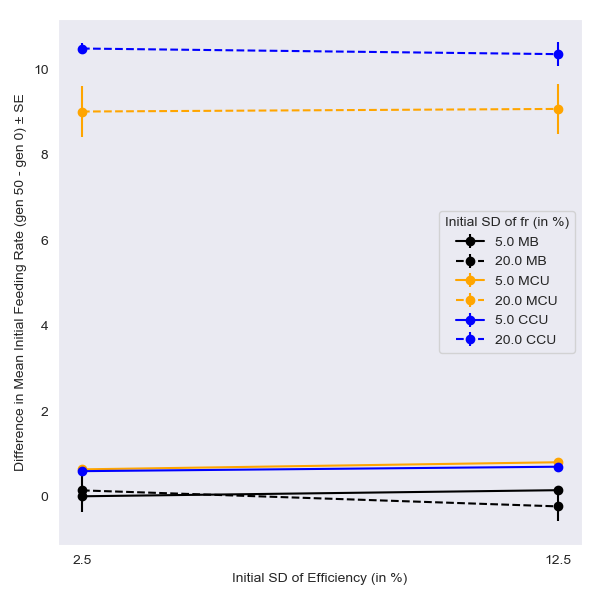
\includegraphics[width=0.5\textwidth]{C5/Figs/ivar/ivar_fr_eff_fr}
  }
  \subfloat{
  \centering
  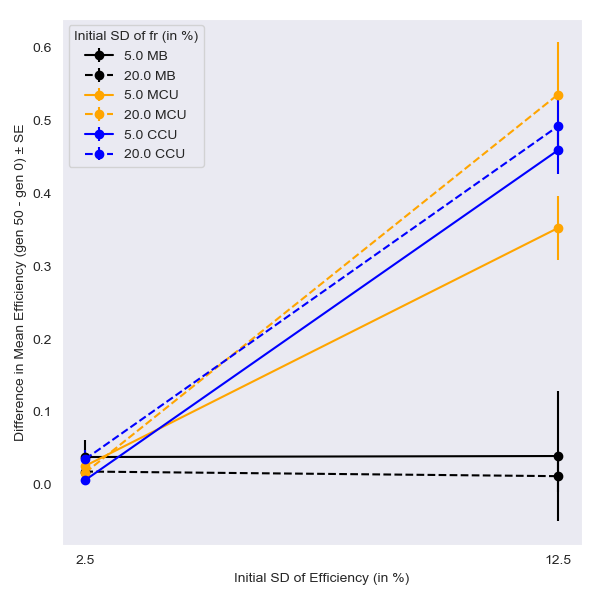
\includegraphics[width=0.5\textwidth]{C5/Figs/ivar/ivar_fr_eff_eff}
  }
  \caption{Effect of initial variation in initial feeding rate and efficiency.}
  \label{fig:ivar_fr_eff}
\end{figure}
\begin{figure}[p]
  \subfloat{
  \centering
  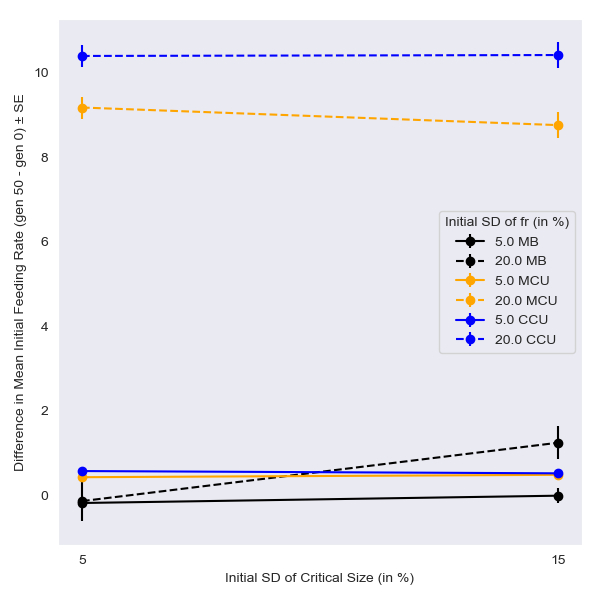
\includegraphics[width=0.5\textwidth]{C5/Figs/ivar/ivar_fr_mc_fr}
  }
  \subfloat{
  \centering
  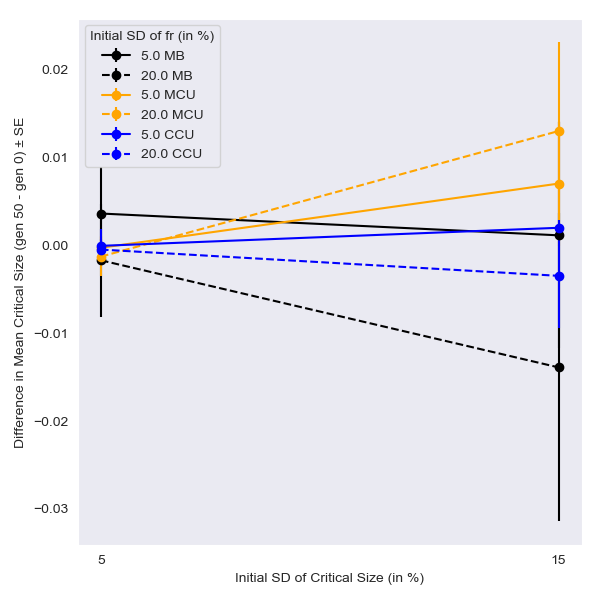
\includegraphics[width=0.5\textwidth]{C5/Figs/ivar/ivar_fr_mc_mc}
  }
  \caption{Effect of initial variation in initial feeding rate and critical size.}
  \label{fig:ivar_fr_mc}
\end{figure}
\newpage

\begin{figure}[t]
  \subfloat{
  \centering
  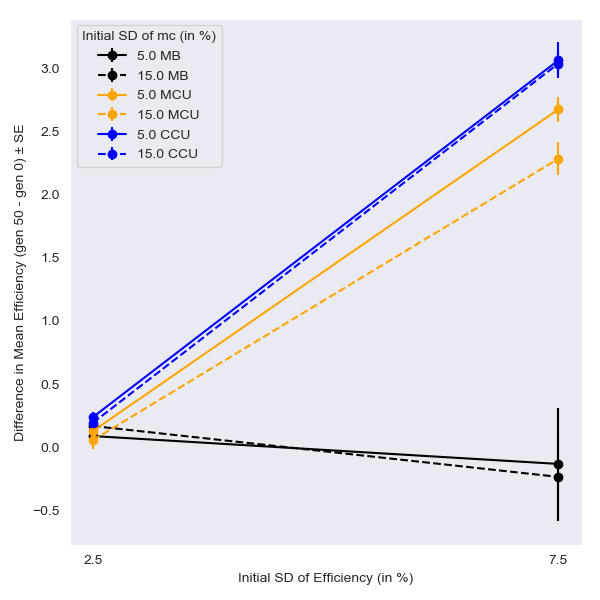
\includegraphics[width=0.5\textwidth]{C5/Figs/ivar/ivar_mc_eff_eff}
  }
  \subfloat{
  \centering
  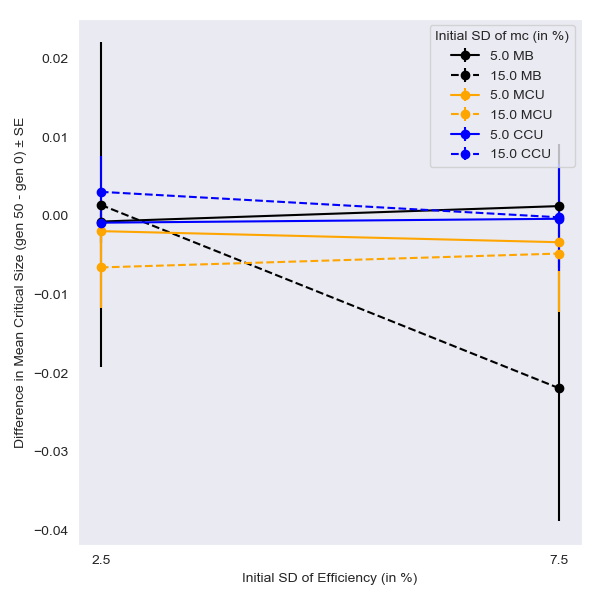
\includegraphics[width=0.5\textwidth]{C5/Figs/ivar/ivar_mc_eff_mc}
  }
  \caption{Effect of initial variation in critical size and efficiency.}
  \label{fig:ivar_mc_eff}
\end{figure}

\section{Heritability of Trait Parameters}
During the inheritance of trait parameters from parents to offspring, the variation in the trait value of offfspring from the parents comes from heritability of that trait parameter. In the model, while assigning the trait value to the offspring from a normal distribution around mid-parent value as mean, the standard deviation ($\omega$) of this distribution is taken as a measure of heritability. This standard deviation, $\omega$, is taken as a certain percentage of mean value of respective parameter at $0^{th}$ generation. Higher the standard deviation, lesser is heritability for that trait parameter. For fixed initial conditions, simulations are performed with varying $\omega$ for combinations of trait parameters across MB, MCU and CCU cultures (see table (no.)). The results from these simulations are plotted similar to initial variation plots (see fig~\ref{fig:omg_fr_eff} - \ref{fig:omg_mc_eff}).\\\\
Results from these simulations show that, initial feeding rate, efficiency and critical size do not show any significant effect of heritability of these trait parameters in MB culture. Higher heritability of initial feeding rate leads to higher mean initial feeding rate in both MCU and CCU culture. This mean feeding rate decreases with decrease in heritability of efficiency in MCU and CCU cultures only when heritability of feeding rate is high, otherwise the interaction with heritability of efficiency is only in CCU culture (fig~\ref{fig:omg_fr_eff}). The only significant difference in mean efficiency is between MCU and CCU culture when heritability of efficiency is less. There is no change in mean critical size due to heritability of these two trait parameters at all densities. Lesser heritability of efficiency also seems to cause increase in mean waste tolerance without any interaction with heritability of feeding rate in all cultures.
\begin{figure}[h]
  \subfloat{
  \centering
  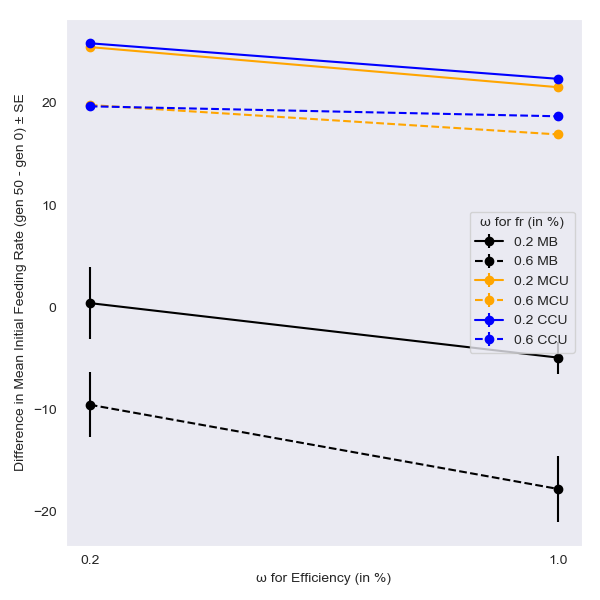
\includegraphics[width=0.5\textwidth]{C5/Figs/omg/omega_fr_eff_fr}
  }
  \subfloat{
  \centering
  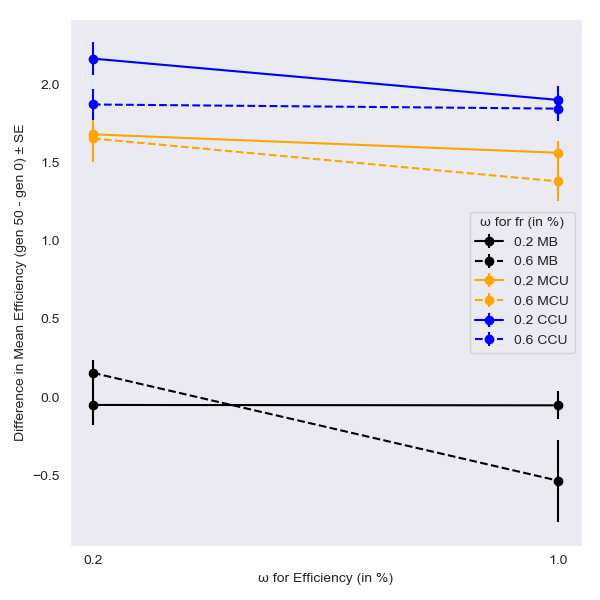
\includegraphics[width=0.5\textwidth]{C5/Figs/omg/omega_fr_eff_eff}
  }\\
  \subfloat{
  \centering
  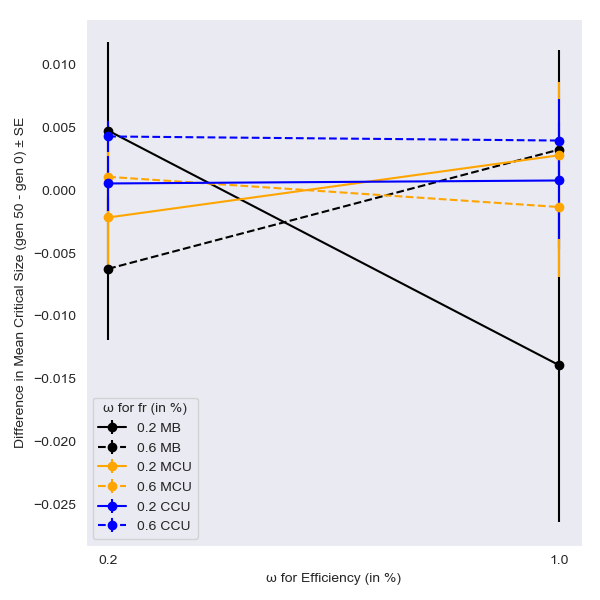
\includegraphics[width=0.5\textwidth]{C5/Figs/omg/omega_fr_eff_mc}
  }
  \subfloat{
  \centering
  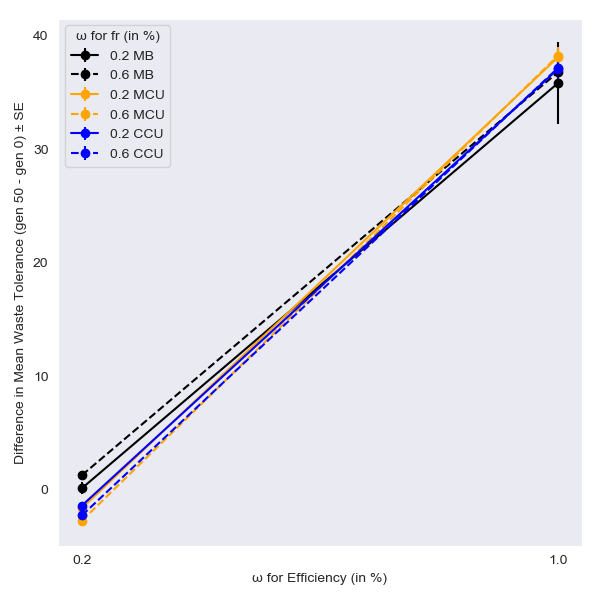
\includegraphics[width=0.5\textwidth]{C5/Figs/omg/omega_fr_eff_wtol}
  }
  \caption{Effect of heritability in initial feeding rate and efficiency on mean trait values at generation 50.}
  \label{fig:omg_fr_eff}
\end{figure}
\newpage

Fig~\ref{fig:omg_fr_mc} shows that heritability of critical size does not affect mean initial feeding rate 
\begin{figure}[p]
  \subfloat{
  \centering
  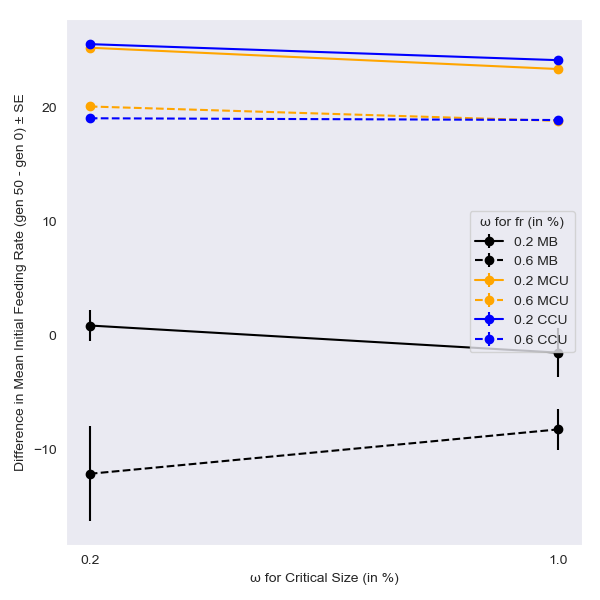
\includegraphics[width=0.5\textwidth]{C5/Figs/omg/omega_fr_mc_fr}
  }
  \subfloat{
  \centering
  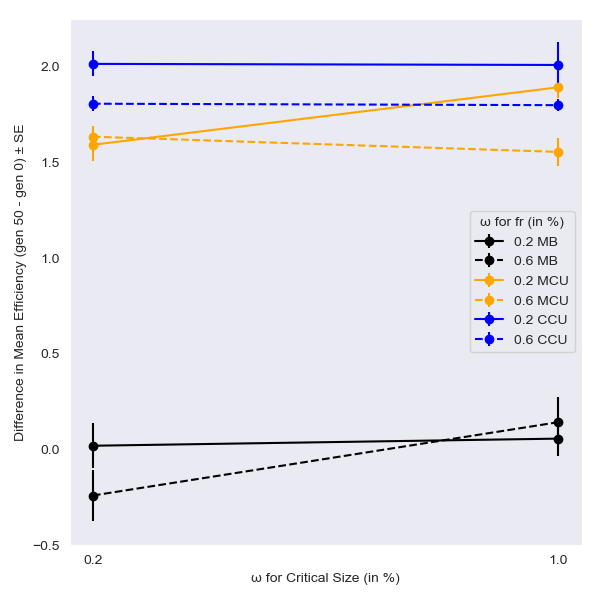
\includegraphics[width=0.5\textwidth]{C5/Figs/omg/omega_fr_mc_eff}
  }\\
  \subfloat{
  \centering
  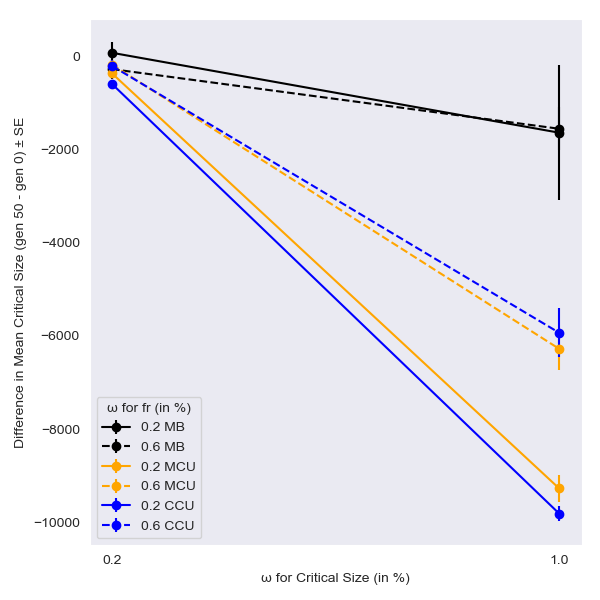
\includegraphics[width=0.5\textwidth]{C5/Figs/omg/omega_fr_mc_mc}
  }
  \subfloat{
  \centering
  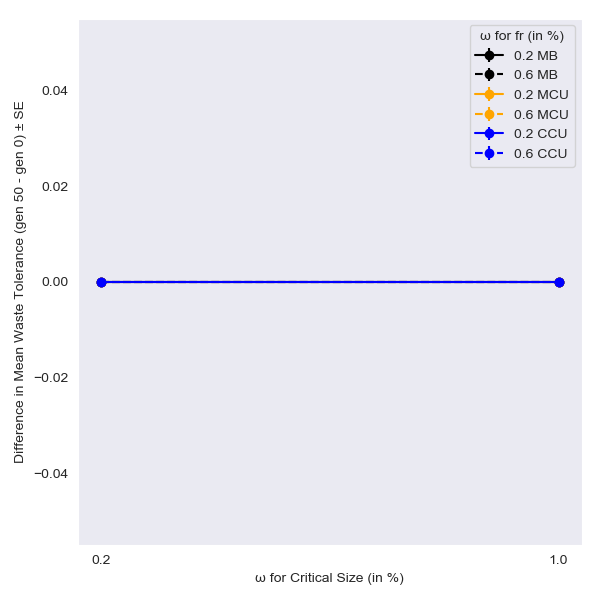
\includegraphics[width=0.5\textwidth]{C5/Figs/omg/omega_fr_mc_wtol}
  }
  \caption{Effect of heritability in initial feeding rate and critical size on mean trait values at generation 50.}
  \label{fig:omg_fr_mc}
\end{figure}
\begin{figure}[p]
  \subfloat{
  \centering
  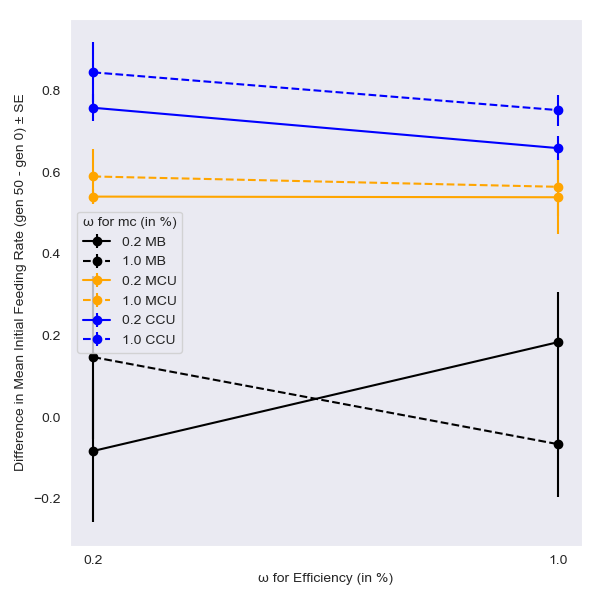
\includegraphics[width=0.5\textwidth]{C5/Figs/omg/omega_mc_eff_fr}
  }
  \subfloat{
  \centering
  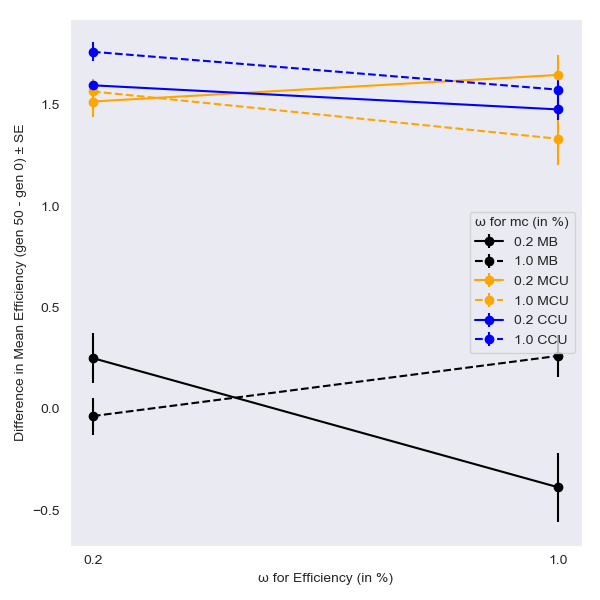
\includegraphics[width=0.5\textwidth]{C5/Figs/omg/omega_mc_eff_eff}
  }\\
  \subfloat{
  \centering
  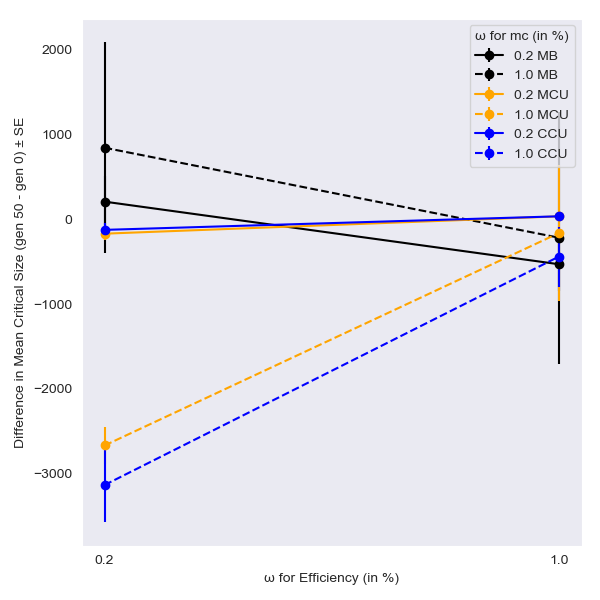
\includegraphics[width=0.5\textwidth]{C5/Figs/omg/omega_mc_eff_mc}
  }
  \subfloat{
  \centering
  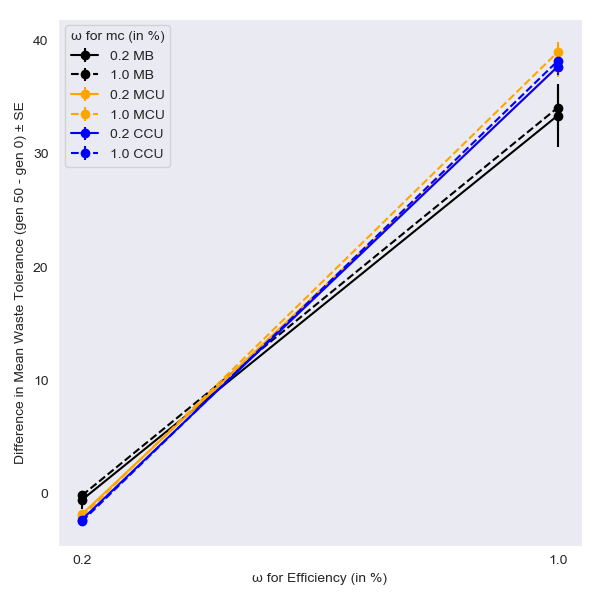
\includegraphics[width=0.5\textwidth]{C5/Figs/omg/omega_mc_eff_wtol}
  }
  \caption{Effect of heritability in critical size and efficiency on mean trait values at generation 50.}
  \label{fig:omg_mc_eff}
\end{figure}
\pagebreak
